
\documentclass[12pt,a4paper]{article}

%========================
% PAQUETES
%========================
\usepackage[utf8]{inputenc}
\usepackage[T1]{fontenc}
\usepackage[spanish,es-tabla]{babel}
\usepackage{amsmath, amssymb, amsfonts}
\usepackage{geometry}
\usepackage{booktabs}
\usepackage{array}
\usepackage{longtable}
\usepackage{multirow}
\usepackage{float}
\usepackage{graphicx}
\usepackage{setspace}
\usepackage{hyperref}
\usepackage{caption}
\usepackage{enumitem}
\usepackage{titlesec}
\usepackage{xcolor}
\usepackage{listings}
\usepackage{fancyhdr}

\geometry{left=2.8cm,right=2.5cm,top=2.5cm,bottom=2.5cm}
\onehalfspacing
\setlength{\parindent}{1.25cm}
\setlength{\parskip}{0.2cm}

\graphicspath{{../codigo/figuras/}{figuras/}}

\hypersetup{
    colorlinks=true,
    linkcolor=blue,
    citecolor=blue,
    urlcolor=blue
}

\titleformat{\section}{\normalfont\Large\bfseries}{\thesection.}{0.5em}{}
\titleformat{\subsection}{\normalfont\large\bfseries}{\thesubsection.}{0.5em}{}
\titleformat{\subsubsection}{\normalfont\normalsize\bfseries}{\thesubsubsection.}{0.5em}{}

%========================
% ESTILO DE CÓDIGO PYTHON
%========================
\definecolor{codegray}{gray}{0.45}
\definecolor{codebg}{rgb}{0.97,0.97,0.97}
\definecolor{codekw}{rgb}{0.10,0.10,0.70}
\definecolor{codecom}{rgb}{0.20,0.50,0.25}
\definecolor{codestr}{rgb}{0.72,0.35,0.05}

\lstdefinestyle{python}{
    language=Python,
    backgroundcolor=\color{codebg},
    basicstyle=\ttfamily\footnotesize,
    keywordstyle=\color{codekw}\bfseries,
    commentstyle=\color{codecom}\itshape,
    stringstyle=\color{codestr},
    showstringspaces=false,
    breaklines=true,
    breakatwhitespace=false,
    frame=single,
    rulecolor=\color{codegray},
    numbers=left,
    numberstyle=\tiny\color{codegray},
    numbersep=8pt,
    tabsize=4,
    captionpos=b,
    inputencoding=utf8,
    extendedchars=true,
    literate=%
      {á}{{\'a}}1 {é}{{\'e}}1 {í}{{\'i}}1 {ó}{{\'o}}1 {ú}{{\'u}}1
      {Á}{{\'A}}1 {É}{{\'E}}1 {Í}{{\'I}}1 {Ó}{{\'O}}1 {Ú}{{\'U}}1
      {ñ}{{\~n}}1 {Ñ}{{\~N}}1 {¿}{{?`}}1 {¡}{{!`}}1
      {×}{{$\times$}}1 {²}{{$^2$}}1 {°}{{$^\circ$}}1 {–}{{-}}1
}
\lstset{style=python}

%========================
% ENCABEZADO Y PIE DE PÁGINA
%========================
\setlength{\headheight}{15pt}
\pagestyle{fancy}
\fancyhf{}
\fancyhead[L]{\small\itshape Examen de Primera Unidad}
\fancyhead[R]{\small\itshape Auditoría estadística UV-C}
\fancyfoot[C]{\thepage}
\fancyfoot[R]{\scriptsize\ttfamily github.com/FranklinUContinental/examen}
\renewcommand{\headrulewidth}{0.4pt}
\renewcommand{\footrulewidth}{0.2pt}

%========================
% DATOS DEL INFORME
%========================
\title{
\textbf{Informe estadístico mejorado del examen de primera unidad}\\
\large Evaluación del diseño experimental y reanálisis estadístico reproducible (con scripts en \textit{Python}) de la investigación sobre radiación UV-C para la inactivación de \textit{Escherichia coli} y \textit{Salmonella typhimurium} en carne de cuy
}

\author{
Curso: Métodos Estadísticos para Investigaciones Experimentales\\
Escuela de Posgrado -- Unidad de Posgrado en Ciencias Físicas y Matemáticas\\
Universidad Nacional de Trujillo
}

\date{\today}

\begin{document}

%========================
% CARÁTULA
%========================
\begin{titlepage}
\centering
\thispagestyle{empty}

{\scshape\Large Universidad Nacional de Trujillo\par}
\vspace{0.35cm}
{\scshape\large Escuela de Posgrado\par}
{\scshape Unidad de Posgrado en Ciencias Físicas y Matemáticas\par}
\vspace{0.6cm}
\rule{\textwidth}{1.0pt}

\vfill

{\Huge\bfseries Informe estadístico del\\examen de primera unidad\par}
\vspace{1.0cm}
{\large\itshape Evaluación del diseño experimental y reanálisis estadístico
reproducible de la investigación sobre radiación UV-C para la inactivación de
\textmd{\textit{Escherichia coli}} y \textmd{\textit{Salmonella typhimurium}}
en carne de cuy\par}

\vspace{1.0cm}
\rule{0.55\textwidth}{0.6pt}

\vfill

{\large
\begin{tabular}{r@{\hspace{1em}}l}
\textbf{Curso:}      & Métodos Estadísticos para Investigaciones Experimentales\\[6pt]
\textbf{Docente:}    & Dr. Roger Reyna Segura\\[6pt]
\textbf{Estudiante:} & Rudy Franklin Condori Quilla\\[6pt]
\textbf{Programa:}   & Posgrado en Ciencias Físicas y Matemáticas\\
\end{tabular}\par}

\vfill

{\small Repositorio del proyecto:\\ \url{https://github.com/FranklinUContinental/examen}\par}
\vspace{0.5cm}
\rule{\textwidth}{1.0pt}
\vspace{0.3cm}
{\large Trujillo -- Perú\par}
{\large \the\year{}\par}

\end{titlepage}

%========================
% NOTA DE LECTURA
%========================
\begin{quote}
\small \textbf{Cómo leer este informe.} Cada modelo se presenta en tres capas: \textbf{(a)~resolución manual} (modelo, hipótesis y, cuando corresponde, cálculo de las sumas de cuadrados), \textbf{(b)~script de Python} que reproduce el análisis, y \textbf{(c)~resultados y explicación}. Además, cada sección sigue una secuencia clara: \textbf{Paso 1} preparar o resumir los datos, \textbf{Paso 2} ejecutar el modelo o gráfico, y \textbf{Paso 3} interpretar los resultados. Todos los valores numéricos provienen del notebook reproducible \texttt{codigo/analisis\_uvc.ipynb} y han sido \emph{verificados contra los datos crudos} del archivo Excel original. Las figuras se generan en \texttt{codigo/figuras/} y se insertan en el apartado correspondiente con su interpretación.
\end{quote}

\newpage
\tableofcontents
\newpage

%========================
\section{Introducción}

El presente informe desarrolla la resolución estadística del examen de primera unidad, cuyo propósito es evaluar críticamente la investigación titulada \textit{Inactivación de patógenos alimentarios en carne de cuy (Cavia porcellus) mediante radiación UV-C}. El problema central consiste en determinar de qué manera la radiación UV-C influye en la inactivación de patógenos alimentarios, específicamente \textit{Escherichia coli} y \textit{Salmonella typhimurium}, inoculados en carne de cuy.

La investigación original plantea que la radiación UV-C reduce la carga microbiana y concluye que la mejor condición de tratamiento corresponde a una exposición de 3 minutos a una distancia de 10 cm. Desde el punto de vista estadístico, es necesario revisar si el diseño declarado, el modelo, las hipótesis, los supuestos y el análisis son coherentes con la estructura real de los datos.

La tesis declara un diseño preexperimental. Sin embargo, los datos presentan una estructura más rica: dos microorganismos, tres tiempos de exposición y tres alturas de irradiación, con repeticiones. Por ello, además del enfoque preexperimental, se analizan los datos mediante el diseño completamente al azar (DCA), el diseño de bloques completamente al azar (DBCA), el diseño factorial y la pertinencia o no del cuadrado latino. Esta versión \emph{mejorada} añade, respecto del informe inicial, la \textbf{reproducción íntegra en Python} de todos los modelos, los \textbf{gráficos} de apoyo y la \textbf{verificación numérica} de cada tabla.

%========================
\section{Objetivos del informe}

\subsection{Objetivo general}

Evaluar si el diseño experimental y los resultados estadísticos de la investigación sobre radiación UV-C en carne de cuy son correctos, y proponer el modelo estadístico más adecuado para el análisis de los datos.

\subsection{Objetivos específicos}

\begin{enumerate}[label=\alph*)]
    \item Revisar críticamente el diseño experimental declarado en la tesis.
    \item Formular modelos estadísticos alternativos aplicables al estudio.
    \item Plantear las hipótesis correspondientes para cada modelo.
    \item Evaluar los supuestos básicos del modelo estadístico seleccionado.
    \item Realizar un nuevo análisis estadístico de los resultados, reproducible en Python.
    \item Comparar los modelos y determinar cuál es el más apropiado.
    \item Formular conclusiones finales sobre la validez estadística de la investigación.
\end{enumerate}

%========================
\section{Descripción del experimento}

La investigación trabaja con carne de cuy contaminada artificialmente con \textit{Escherichia coli} y \textit{Salmonella typhimurium}. Los tratamientos de radiación UV-C se organizaron combinando los factores siguientes:

\begin{table}[H]
\centering
\caption{Factores experimentales considerados en la investigación}
\begin{tabular}{lll}
\toprule
\textbf{Factor} & \textbf{Niveles} & \textbf{Tipo de factor}\\
\midrule
Microorganismo & \textit{E. coli}, \textit{S. typhimurium} & Factor biológico (2)\\
Tiempo de exposición & 1, 3 y 5 minutos & Factor experimental (3)\\
Altura o distancia & 5, 10 y 20 cm & Factor experimental (3)\\
Repetición & M1, M2, M3, M4 & Error experimental (4)\\
\bottomrule
\end{tabular}
\end{table}

La variable respuesta es el recuento de microorganismos sobrevivientes en placa después del tratamiento UV-C. El número total de observaciones tratadas es $2\times3\times3\times4=72$, más los controles $T(0)\text{--}H(0)$ (media $235$ para \textit{E. coli} y $240{,}25$ para \textit{S. typhimurium}). Para datos microbiológicos se recomienda además trabajar en escala logarítmica:

\[
Y = \log_{10}(\text{UFC/g}), \qquad
R = \log_{10}(N_0) - \log_{10}(N),
\]

donde \(N_0\) es la carga microbiana inicial y \(N\) la posterior al tratamiento. Los datos crudos completos se documentan en \texttt{enunciado.md} y en formato ordenado en \texttt{codigo/datos\_uvc.csv}.

\subsection{Medias de recuento por tratamiento}

\begin{table}[H]
\centering
\caption{Medias de recuento (tiempo $\times$ altura). En negrita el mínimo (3 min -- 10 cm).}
\begin{tabular}{lccc|ccc}
\toprule
 & \multicolumn{3}{c|}{\textit{E. coli}} & \multicolumn{3}{c}{\textit{S. typhimurium}}\\
\textbf{min \textbackslash{} cm} & 5 & 10 & 20 & 5 & 10 & 20\\
\midrule
1 & 9.50 & 12.00 & 15.00 & 11.50 & 16.25 & 18.50\\
3 & 11.75 & \textbf{6.75} & 13.50 & 11.25 & \textbf{6.00} & 14.75\\
5 & 16.50 & 13.50 & 12.50 & 17.00 & 13.00 & 12.00\\
\bottomrule
\end{tabular}
\end{table}

%========================
\section{Evaluación crítica del diseño original}

La tesis clasifica la investigación como preexperimental. En un diseño preexperimental se evalúa un solo grupo con medición antes y después del tratamiento, sin estructura factorial:

\[
O_1 \quad X \quad O_2
\]

Sin embargo, la estructura real de los datos no corresponde a un esquema antes--después. El estudio no solo busca determinar si la UV-C reduce la carga microbiana, sino también cómo influyen el tiempo y la altura. Por tanto, el diseño declarado es insuficiente.

\subsection{Observaciones críticas}

\begin{enumerate}[label=\alph*)]
    \item El diseño preexperimental no permite evaluar la interacción tiempo--altura.
    \item Hay dos factores experimentales principales: tiempo y altura.
    \item Se incluyen dos microorganismos, por lo que cabe un factorial de tres factores.
    \item La tesis debió declarar un diseño completamente al azar con arreglo factorial.
    \item La hipótesis original es ambigua (``influye significativamente o no''): mezcla $H_1$ con $H_0$.
    \item El análisis debe considerar normalidad, homogeneidad de varianzas e independencia.
\end{enumerate}

%========================
\section{Metodología computacional y datos}

Todo el reanálisis es reproducible. El entorno emplea \texttt{pandas}, \texttt{numpy}, \texttt{scipy}, \texttt{statsmodels}, \texttt{matplotlib} y \texttt{seaborn}. Los datos se cargan en formato ordenado (\textit{tidy}): una fila por observación con las columnas \texttt{microorganismo}, \texttt{tiempo}, \texttt{altura}, \texttt{rep}, \texttt{recuento} y \texttt{trat}.

\begin{lstlisting}[caption={Carga de datos y entorno de trabajo.}]
import numpy as np, pandas as pd
import scipy.stats as stats
import statsmodels.api as sm
from statsmodels.formula.api import ols
from statsmodels.stats.anova import anova_lm
from statsmodels.stats.multicomp import pairwise_tukeyhsd

df = pd.read_csv("datos_uvc.csv")   # 72 obs: microorganismo, tiempo, altura, rep, recuento, trat
control = {"E. coli":[225,240,245,230], "S. typhimurium":[247,245,236,233]}
N0 = {org: np.mean(v) for org, v in control.items()}
\end{lstlisting}

%========================
\section{Estadística descriptiva y exploración gráfica}

\begin{lstlisting}[caption={Resumen descriptivo y porcentaje de inactivación.}]
resumen = (df.groupby(["microorganismo","tiempo","altura"]).recuento
             .agg(media="mean", sd="std").reset_index())
resumen["pct_inactivacion"] = resumen.apply(
    lambda r: 100*(1 - r.media/N0[r.microorganismo]), axis=1)
\end{lstlisting}

El mínimo absoluto de recuento, en ambos patógenos, es la celda \textbf{3 min -- 10 cm}. Todos los tratamientos superan el $94\%$ de inactivación respecto al control.

\begin{figure}[H]
\centering
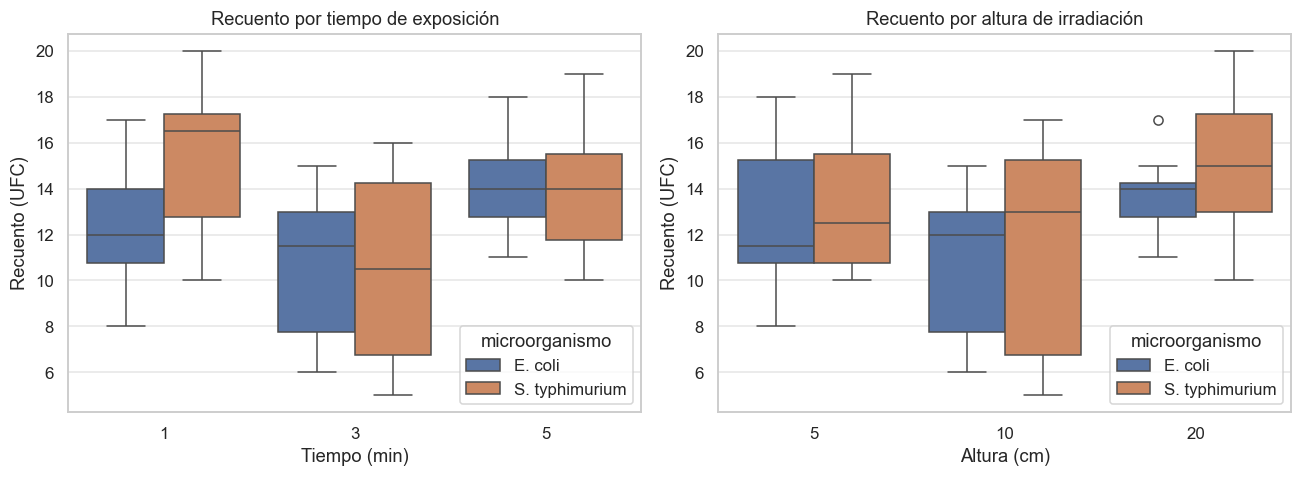
\includegraphics[width=0.95\textwidth]{01_boxplots_factores.png}
\caption{Distribución de recuentos por tiempo de exposición y por altura de irradiación.}
\end{figure}

\begin{figure}[H]
\centering
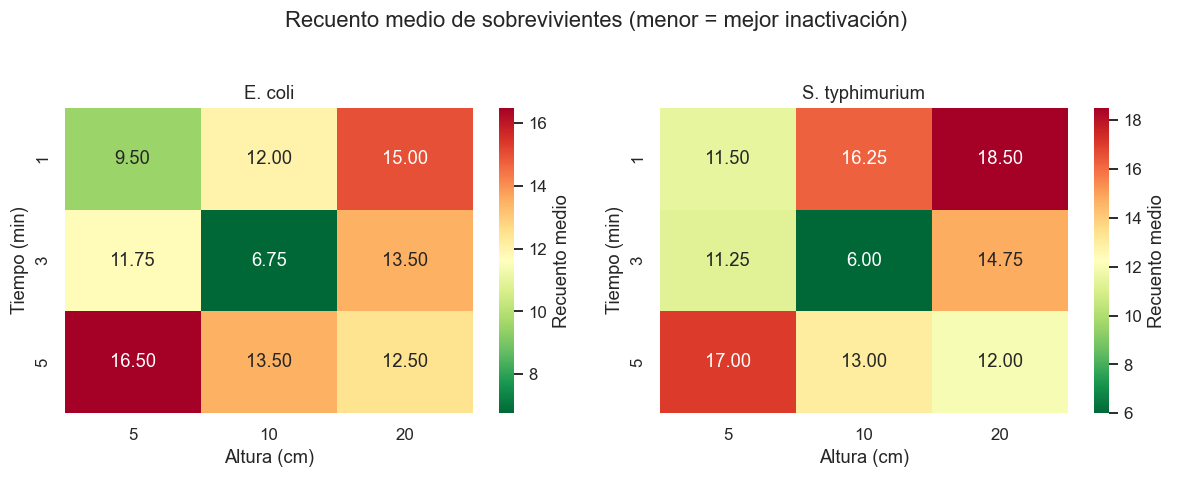
\includegraphics[width=0.95\textwidth]{02_heatmaps_medias.png}
\caption{Mapa de calor de medias (tiempo $\times$ altura). La celda 3 min -- 10 cm (verde oscuro) es el mínimo. El patrón anticipa una interacción.}
\end{figure}

\begin{figure}[H]
\centering
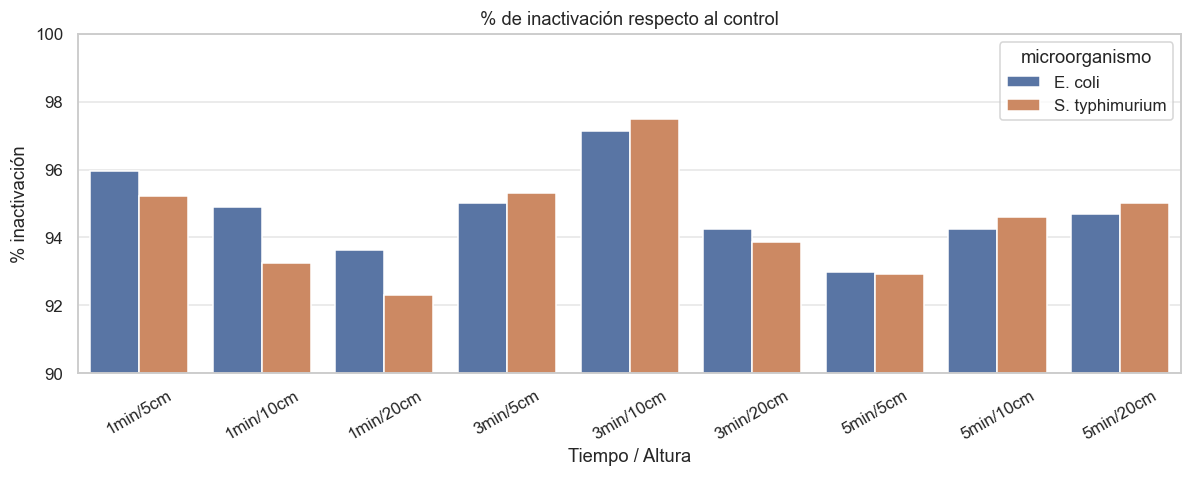
\includegraphics[width=0.95\textwidth]{03_pct_inactivacion.png}
\caption{Porcentaje de inactivación por tratamiento (todos superan el 94\%).}
\end{figure}

%========================
\section{Modelo 1: Diseño preexperimental}

\subsection{Resolución manual}

\[
Y_{ij} = \mu + \tau_i + e_{ij}
\]

con $\mu$ media general, $\tau_i$ efecto del tratamiento UV-C (control vs.\ tratado) y $e_{ij}$ error. Hipótesis:

\[
H_0: \mu_{\text{control}} = \mu_{\text{tratado}}, \qquad
H_1: \mu_{\text{control}} \neq \mu_{\text{tratado}}.
\]

Se contrasta con un $t$ de Welch (control: $n=4$; tratado: $n=36$) por microorganismo.

\subsection{Script en Python}

\begin{lstlisting}[caption={Prueba t de control vs.\ tratado.}]
for org in df.microorganismo.unique():
    c = np.array(control[org], float)
    t = df[df.microorganismo==org].recuento.values.astype(float)
    tstat, p = stats.ttest_ind(c, t, equal_var=False)   # Welch
    print(org, c.mean(), t.mean(), tstat, p)
\end{lstlisting}

\subsection{Resultados}

\begin{table}[H]
\centering
\caption{Modelo preexperimental: control vs.\ tratado.}
\begin{tabular}{lrrrrr}
\toprule
\textbf{Microorganismo} & \textbf{Media ctrl.} & \textbf{Media trat.} & \textbf{Reducción} & \textbf{$t$} & \textbf{$p$}\\
\midrule
\textit{E. coli} & 235.00 & 12.33 & 94.75\% & 48.50 & $1.6\times10^{-5}$\\
\textit{S. typhimurium} & 240.25 & 13.36 & 94.44\% & 65.58 & $3.9\times10^{-6}$\\
\bottomrule
\end{tabular}
\end{table}

\subsection{Explicación}

Se rechaza $H_0$ con holgura: la UV-C \textbf{sí} reduce la carga microbiana ($\approx 95\%$). Pero el modelo no indica \emph{cuál} tiempo o altura es óptimo ni evalúa la interacción. Sirve como análisis exploratorio, no como análisis principal.

%========================
\section{Modelo 2: Diseño completamente al azar (DCA)}

\subsection{Resolución manual}

Cada combinación tiempo--altura es un tratamiento ($t=9$, $r=4$, $N=36$):

\[
Y_{ij} = \mu + \tau_i + e_{ij}, \qquad H_0: \mu_1=\mu_2=\cdots=\mu_9.
\]

Con $T_i$ el total del tratamiento $i$, $G$ el gran total y $C=G^2/N$:

\[
SC_{trat}=\sum_i \frac{T_i^2}{r}-C,\quad
SC_{tot}=\sum Y^2-C,\quad
SC_{error}=SC_{tot}-SC_{trat}.
\]

Para \textit{E. coli}: $G=444$, $C=444^2/36=5476$, $\sum_i T_i^2/r = 5743{,}5$, $\sum Y^2 = 5782$. Por tanto:

\[
SC_{tot}=306{,}0,\quad SC_{trat}=267{,}5,\quad SC_{error}=38{,}5,
\]
\[
F=\frac{267{,}5/8}{38{,}5/27}=\frac{33{,}44}{1{,}426}=23{,}45.
\]

\subsection{Script en Python}

\begin{lstlisting}[caption={ANOVA del DCA por microorganismo.}]
for org in df.microorganismo.unique():
    sub = df[df.microorganismo==org]
    modelo = ols("recuento ~ C(trat)", data=sub).fit()
    print(org, anova_lm(modelo, typ=2))
\end{lstlisting}

\subsection{Resultados}

\begin{table}[H]
\centering
\caption{ANOVA DCA para \textit{E. coli}.}
\begin{tabular}{lrrrrr}
\toprule
\textbf{Fuente} & \textbf{SC} & \textbf{gl} & \textbf{CM} & \textbf{F} & \textbf{p-valor}\\
\midrule
Tratamientos & 267.50 & 8 & 33.44 & 23.45 & $<0.001$\\
Error & 38.50 & 27 & 1.43 & &\\
Total & 306.00 & 35 & & &\\
\bottomrule
\end{tabular}
\end{table}

\begin{table}[H]
\centering
\caption{ANOVA DCA para \textit{Salmonella typhimurium}.}
\begin{tabular}{lrrrrr}
\toprule
\textbf{Fuente} & \textbf{SC} & \textbf{gl} & \textbf{CM} & \textbf{F} & \textbf{p-valor}\\
\midrule
Tratamientos & 456.06 & 8 & 57.01 & 26.42 & $<0.001$\\
Error & 58.25 & 27 & 2.16 & &\\
Total & 514.31 & 35 & & &\\
\bottomrule
\end{tabular}
\end{table}

\subsection{Explicación}

Se rechaza $H_0$ en ambos patógenos: hay diferencias significativas entre tratamientos. Limitación: el DCA no descompone si la diferencia proviene del tiempo, de la altura o de su interacción. Es mejor que el preexperimental, pero no es el más informativo.

%========================
\section{Modelo 3: Diseño de bloques completamente al azar (DBCA)}

\subsection{Resolución manual}

Si las réplicas M1--M4 fueran bloques (días, lotes, placas):

\[
Y_{ij} = \mu + \tau_i + \beta_j + e_{ij},
\]

con hipótesis para tratamientos ($\mu_1=\cdots=\mu_9$) y para bloques ($\beta_1=\cdots=\beta_4=0$). Se añade $SC_{bloque}=\sum_j T_{\cdot j}^2/t - C$ y el error pierde 3 grados de libertad.

\subsection{Script en Python}

\begin{lstlisting}[caption={ANOVA del DBCA (bloque = réplica).}]
modelo = ols("recuento ~ C(trat) + C(rep)", data=sub).fit()
anova_lm(modelo, typ=2)
\end{lstlisting}

\subsection{Resultados}

\begin{table}[H]
\centering
\caption{ANOVA DBCA para \textit{E. coli}.}
\begin{tabular}{lrrrr}
\toprule
\textbf{Fuente} & \textbf{SC} & \textbf{gl} & \textbf{F} & \textbf{p-valor}\\
\midrule
Tratamientos & 267.50 & 8 & 22.54 & $<0.001$\\
Bloques (réplica) & 2.89 & 3 & 0.65 & 0.591\\
Error & 35.61 & 24 & &\\
Total & 306.00 & 35 & &\\
\bottomrule
\end{tabular}
\end{table}

\begin{table}[H]
\centering
\caption{ANOVA DBCA para \textit{Salmonella typhimurium}.}
\begin{tabular}{lrrrr}
\toprule
\textbf{Fuente} & \textbf{SC} & \textbf{gl} & \textbf{F} & \textbf{p-valor}\\
\midrule
Tratamientos & 456.06 & 8 & 24.65 & $<0.001$\\
Bloques (réplica) & 2.75 & 3 & 0.40 & 0.757\\
Error & 55.50 & 24 & &\\
Total & 514.31 & 35 & &\\
\bottomrule
\end{tabular}
\end{table}

\subsection{Explicación}

Los bloques \textbf{no son significativos} ($p=0{,}591$ y $0{,}757$): las réplicas no representan una fuente sistemática de variación. Como la tesis tampoco justifica un bloqueo real, el DBCA no aporta sobre el DCA (e incluso pierde grados de libertad del error).

%========================
\section{Modelo 4: Diseño cuadrado latino (no aplica)}

\subsection{Resolución manual}

\[
Y_{ijk} = \mu + \tau_i + \rho_j + \gamma_k + e_{ijk}.
\]

El cuadrado latino exige \textbf{dos} factores de bloqueo cruzados (filas y columnas) y un número igual de tratamientos, filas y columnas. No corresponde aquí porque el tiempo y la altura no son bloques, sino factores de interés, y su \textbf{interacción} es justamente el objeto de estudio.

\subsection{Demostración numérica en Python}

\begin{lstlisting}[caption={Comparación de un modelo aditivo (estilo cuadrado latino) vs.\ con interacción.}]
aditivo  = ols("recuento ~ C(tiempo) + C(altura)", data=sub).fit()  # sin interaccion
completo = ols("recuento ~ C(tiempo) * C(altura)", data=sub).fit()
print(aditivo.ssr, completo.ssr)   # E. coli: 179.83 vs 38.50
\end{lstlisting}

\subsection{Explicación}

Para \textit{E. coli}, el modelo aditivo deja $SC_{error}=179{,}83$, frente a $38{,}50$ del modelo con interacción. Es decir, un diseño tipo cuadrado latino enviaría al error $179{,}83-38{,}50=141{,}33$ unidades de variación que en realidad son la \textbf{interacción tiempo--altura}, inflando el error y ocultando el efecto más importante. \textbf{El cuadrado latino es inaplicable} y conduciría a interpretaciones erróneas.

%========================
\section{Modelo 5: Diseño factorial 3 \texorpdfstring{$\times$}{x} 3 por microorganismo}

\subsection{Resolución manual}

\[
Y_{ijk} = \mu + \alpha_i + \beta_j + (\alpha\beta)_{ij} + e_{ijk},
\]

con $\alpha$ = tiempo y $\beta$ = altura. Descompone $SC_{trat}$ del DCA:
$SC_{trat}=SC_{tiempo}+SC_{altura}+SC_{tiempo\times altura}$. Tres juegos de hipótesis: $H_0:\alpha_i=0$ (tiempo), $H_0:\beta_j=0$ (altura) y $H_0:(\alpha\beta)_{ij}=0$ (interacción).

\subsection{Script en Python}

\begin{lstlisting}[caption={ANOVA factorial 3x3 por microorganismo.}]
for org in df.microorganismo.unique():
    sub = df[df.microorganismo==org]
    modelo = ols("recuento ~ C(tiempo) * C(altura)", data=sub).fit()
    print(org, anova_lm(modelo, typ=2), "R2=", modelo.rsquared)
\end{lstlisting}

\subsection{Resultados}

\begin{table}[H]
\centering
\caption{ANOVA factorial 3 $\times$ 3 para \textit{E. coli} ($R^2=0{,}874$).}
\begin{tabular}{lrrrr}
\toprule
\textbf{Fuente} & \textbf{SC} & \textbf{gl} & \textbf{F} & \textbf{p-valor}\\
\midrule
Tiempo & 74.00 & 2 & 25.95 & $<0.001$\\
Altura & 52.17 & 2 & 18.29 & $<0.001$\\
Tiempo $\times$ Altura & 141.33 & 4 & 24.78 & $<0.001$\\
Error & 38.50 & 27 & &\\
Total & 306.00 & 35 & &\\
\bottomrule
\end{tabular}
\end{table}

\begin{table}[H]
\centering
\caption{ANOVA factorial 3 $\times$ 3 para \textit{Salmonella typhimurium} ($R^2=0{,}887$).}
\begin{tabular}{lrrrr}
\toprule
\textbf{Fuente} & \textbf{SC} & \textbf{gl} & \textbf{F} & \textbf{p-valor}\\
\midrule
Tiempo & 142.72 & 2 & 33.08 & $<0.001$\\
Altura & 66.89 & 2 & 15.50 & $<0.001$\\
Tiempo $\times$ Altura & 246.44 & 4 & 28.56 & $<0.001$\\
Error & 58.25 & 27 & &\\
Total & 514.31 & 35 & &\\
\bottomrule
\end{tabular}
\end{table}

Nótese que $74{,}00+52{,}17+141{,}33=267{,}50=SC_{trat}$ del DCA: el factorial \emph{descompone} lo que el DCA dejaba agregado.

\begin{figure}[H]
\centering
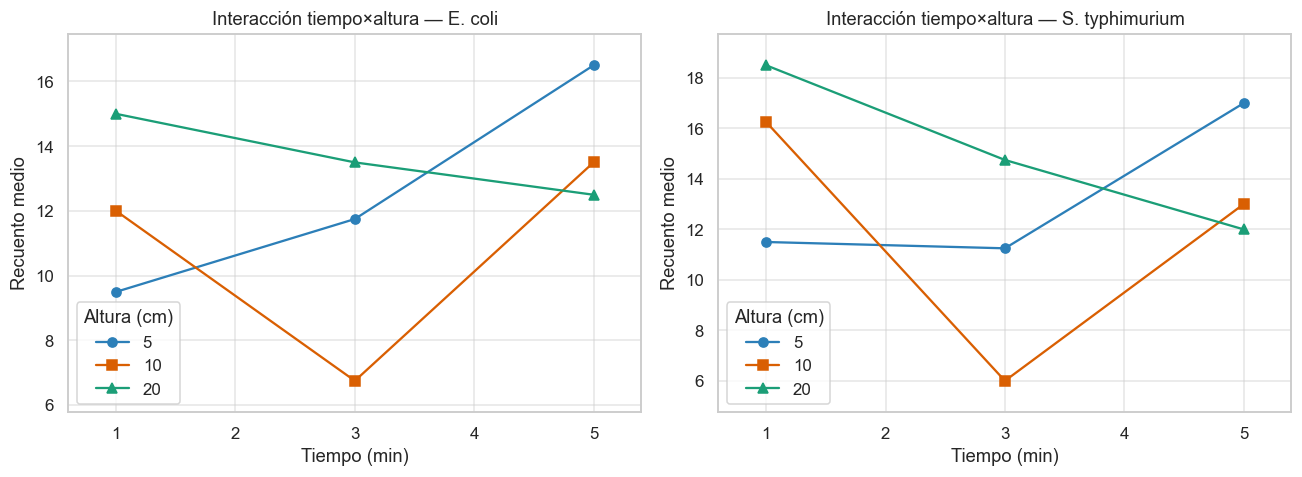
\includegraphics[width=0.95\textwidth]{04_interaccion_tiempo_altura.png}
\caption{Gráficos de interacción tiempo $\times$ altura. Las líneas se cruzan: la curva de 10 cm cae fuerte a los 3 min (óptimo), mientras que 5 cm y 20 cm se comportan distinto.}
\end{figure}

\subsection{Explicación}

Tiempo, altura y su interacción son significativos en ambos patógenos. La interacción domina (mayor $SC$): no puede elegirse el mejor tiempo ignorando la altura. El óptimo es una \textbf{combinación}: 3 min -- 10 cm.

%========================
\section{Modelo 6: Diseño factorial 2 \texorpdfstring{$\times$}{x} 3 \texorpdfstring{$\times$}{x} 3 (recomendado)}

\subsection{Resolución manual}

\[
Y_{ijkl} = \mu + A_i + B_j + C_k + (AB)_{ij} + (AC)_{ik} + (BC)_{jk} + (ABC)_{ijk} + e_{ijkl},
\]

con $A$ = microorganismo, $B$ = tiempo, $C$ = altura. Cada efecto e interacción tiene como $H_0$ que sus términos son nulos. Con $N=72$, los grados de libertad del error son $72-1-(1+2+2+2+2+4+4)=54$.

\subsection{Script en Python}

\begin{lstlisting}[caption={ANOVA factorial 2x3x3 (modelo completo).}]
modelo_full = ols("recuento ~ C(microorganismo) * C(tiempo) * C(altura)", data=df).fit()
anova_lm(modelo_full, typ=2)
\end{lstlisting}

\subsection{Resultados}

\begin{table}[H]
\centering
\caption{ANOVA factorial 2 $\times$ 3 $\times$ 3 ($R^2=0{,}885$; $R^2_{adj}=0{,}848$).}
\begin{tabular}{lrrrr}
\toprule
\textbf{Fuente} & \textbf{SC} & \textbf{gl} & \textbf{F} & \textbf{p-valor}\\
\midrule
Microorganismo (A) & 19.01 & 1 & 10.61 & 0.0019\\
Tiempo (B) & 172.19 & 2 & 48.05 & $<0.001$\\
Altura (C) & 117.36 & 2 & 32.75 & $<0.001$\\
A $\times$ B & 44.53 & 2 & 12.43 & $<0.001$\\
A $\times$ C & 1.69 & 2 & 0.47 & 0.626\\
B $\times$ C (tiempo $\times$ altura) & 378.14 & 4 & 52.76 & $<0.001$\\
A $\times$ B $\times$ C & 9.64 & 4 & 1.34 & 0.265\\
Error & 96.75 & 54 & &\\
\bottomrule
\end{tabular}
\end{table}

\subsection{Explicación}

Son significativos: microorganismo, tiempo, altura, la interacción microorganismo--tiempo y, de forma dominante, la \textbf{interacción tiempo--altura} ($F=52{,}76$, la mayor de todas). No son significativas microorganismo--altura ni la interacción triple. Es el modelo \textbf{más completo y recomendable}: integra todo en un único análisis y confirma que el óptimo se elige por combinación de niveles.

%========================
\section{Evaluación de supuestos del modelo seleccionado}

Sobre los residuos del modelo $2\times3\times3$.

\begin{lstlisting}[caption={Normalidad (Shapiro--Wilk) y homocedasticidad (Levene).}]
W, p = stats.shapiro(modelo_full.resid)                        # normalidad
grupos = [g.recuento.values for _, g in df.groupby(["microorganismo","trat"])]
stat, p = stats.levene(*grupos, center="median")               # homocedasticidad
\end{lstlisting}

\begin{table}[H]
\centering
\caption{Prueba de normalidad de residuos (Shapiro--Wilk).}
\begin{tabular}{lcc}
\toprule
\textbf{Análisis} & \textbf{p-valor} & \textbf{Decisión}\\
\midrule
Modelo global & 0.068 & No se rechaza normalidad\\
\textit{E. coli} & 0.032 & Normalidad dudosa\\
\textit{S. typhimurium} & 0.325 & No se rechaza normalidad\\
\bottomrule
\end{tabular}
\end{table}

\begin{table}[H]
\centering
\caption{Prueba de homogeneidad de varianzas (Levene, 9 tratamientos).}
\begin{tabular}{lcc}
\toprule
\textbf{Análisis} & \textbf{p-valor} & \textbf{Decisión}\\
\midrule
Modelo global & 0.915 & Se cumple homogeneidad\\
\textit{E. coli} & 0.943 & Se cumple homogeneidad\\
\textit{S. typhimurium} & 0.727 & Se cumple homogeneidad\\
\bottomrule
\end{tabular}
\end{table}

\begin{figure}[H]
\centering
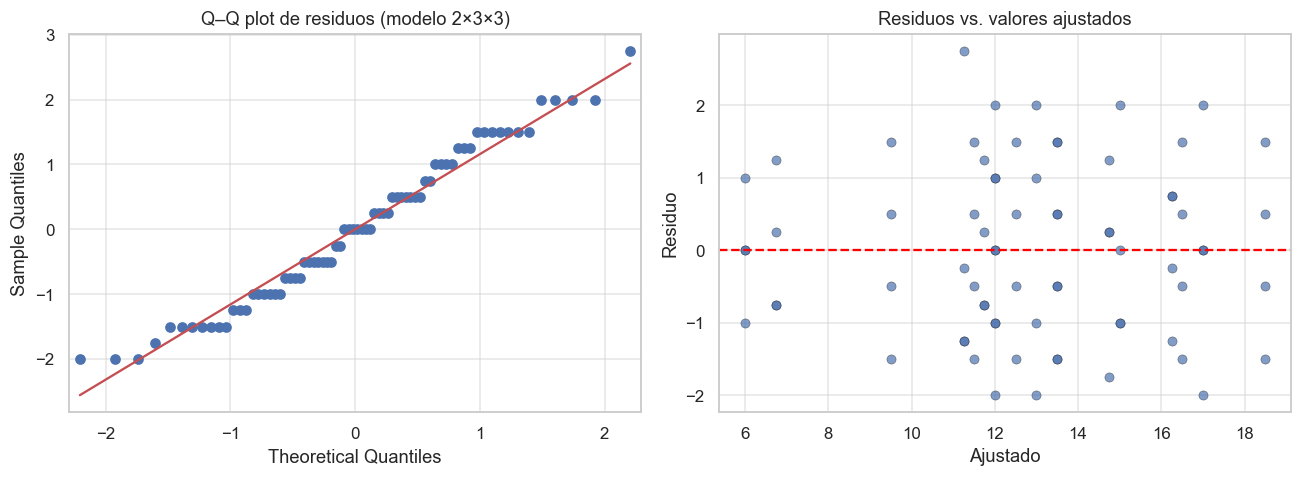
\includegraphics[width=0.95\textwidth]{05_diagnostico_residuos.png}
\caption{Q--Q plot (los puntos siguen la recta) y residuos vs.\ valores ajustados (nube sin patrón ni embudo): los supuestos se satisfacen razonablemente.}
\end{figure}

\begin{itemize}
    \item \textbf{Independencia:} depende de la aleatorización; la tesis no la describe, por lo que debe garantizarse desde el diseño.
    \item \textbf{Normalidad:} global aceptable; en \textit{E. coli} es dudosa, lo que sugiere la transformación $Y^\ast=\log_{10}(Y)$ o la reducción logarítmica $R=\log_{10}(N_0)-\log_{10}(N)$.
    \item \textbf{Homocedasticidad:} se cumple holgadamente.
    \item \textbf{Aditividad:} hay interacción tiempo--altura significativa; debe interpretarse por combinación de niveles.
\end{itemize}

%========================
\section{Comparaciones múltiples (Tukey HSD)}

Como la interacción tiempo--altura es significativa, el tratamiento óptimo se identifica por combinación. Se aplica Tukey sobre los 9 tratamientos por microorganismo.

\begin{lstlisting}[caption={Comparaciones múltiples de Tukey.}]
for org in df.microorganismo.unique():
    sub = df[df.microorganismo==org]
    print(pairwise_tukeyhsd(sub.recuento, sub.trat, alpha=0.05).summary())
\end{lstlisting}

\begin{table}[H]
\centering
\caption{Resumen de Tukey HSD por microorganismo (etiquetas T\textit{tiempo}\_H\textit{altura}).}
\begin{tabular}{lccc}
\toprule
\textbf{Microorganismo} & \textbf{Mejor (menor recuento)} & \textbf{Peor} & \textbf{Pares signif.}\\
\midrule
\textit{E. coli} & T3\_H10 (3 min--10 cm): 6.75 & T5\_H5: 16.50 & 19/36\\
\textit{S. typhimurium} & T3\_H10 (3 min--10 cm): 6.00 & T1\_H20: 18.50 & 21/36\\
\bottomrule
\end{tabular}
\end{table}

\begin{figure}[H]
\centering
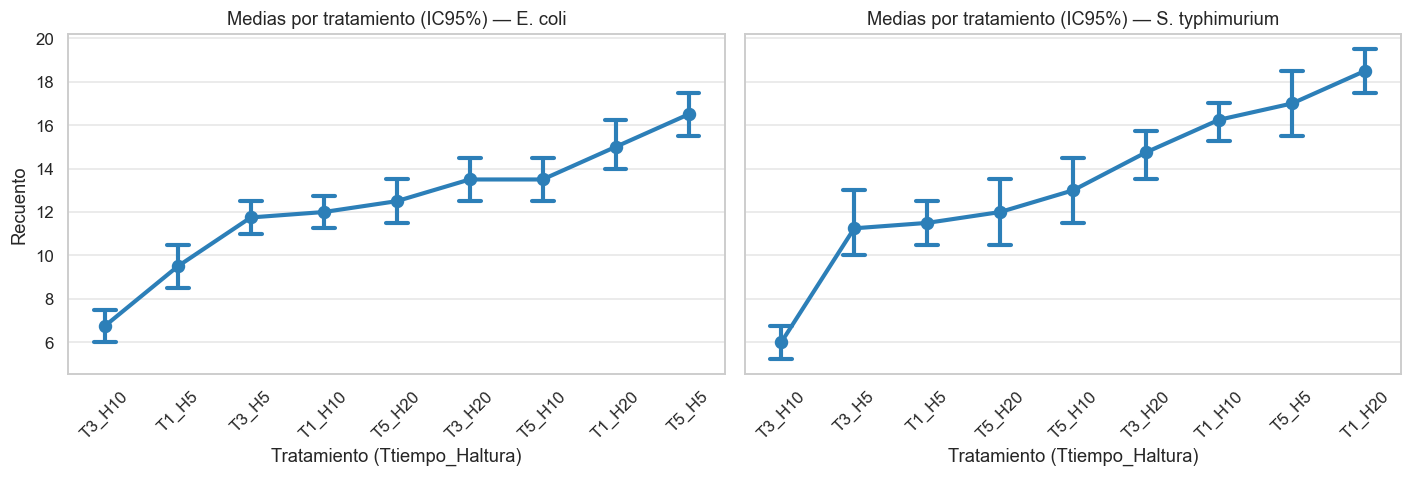
\includegraphics[width=0.98\textwidth]{06_medias_tukey.png}
\caption{Medias por tratamiento con intervalos de confianza al 95\%, ordenadas. El tratamiento 3 min -- 10 cm queda aislado en el extremo inferior en ambos patógenos.}
\end{figure}

Tukey confirma estadísticamente que \textbf{3 min -- 10 cm} produce el menor recuento y difiere de la mayoría de los demás tratamientos: respalda la ``mejor condición'' declarada por la tesis.

%========================
\section{Comparación general de modelos}

\begin{longtable}{p{3.2cm}p{2.2cm}p{4cm}p{4cm}}
\caption{Comparación de modelos estadísticos evaluados.}\\
\toprule
\textbf{Modelo} & \textbf{Aplicabilidad} & \textbf{Resultado principal} & \textbf{Evaluación}\\
\midrule
\endfirsthead
\toprule
\textbf{Modelo} & \textbf{Aplicabilidad} & \textbf{Resultado principal} & \textbf{Evaluación}\\
\midrule
\endhead
Preexperimental & Parcial & Detecta reducción global ($\approx 95\%$) & Insuficiente: no evalúa tiempo, altura ni interacción\\
DCA & Sí & Tratamientos significativos ($p<0.001$) & Válido, pero no separa efectos principales\\
DBCA & Condicional & Tratamientos signif.; bloques no ($p=0.59/0.76$) & No mejora al DCA; bloqueo injustificado\\
Cuadrado latino & No & No corresponde a la estructura & Confundiría la interacción con el error\\
Factorial 3 $\times$ 3 & Sí & Tiempo, altura e interacción significativos & Muy adecuado por microorganismo\\
Factorial 2 $\times$ 3 $\times$ 3 & Sí & Evalúa microorganismo, tiempo, altura e interacciones & \textbf{Modelo recomendado (más completo)}\\
\bottomrule
\end{longtable}

%========================
\section{Discusión}

La radiación UV-C \textbf{sí} reduce la carga microbiana ($\approx 95\%$ en todos los tratamientos). Pero la solidez de la conclusión depende del modelo: el preexperimental solo detecta la reducción global; el DCA y el DBCA confirman diferencias entre tratamientos sin descomponerlas; el cuadrado latino es inaplicable. El factorial revela lo esencial: el efecto del tiempo \emph{depende} de la altura (interacción tiempo--altura, el término de mayor suma de cuadrados). Por eso el óptimo no es ``el mejor tiempo'' ni ``la mejor altura'' por separado, sino la \textbf{combinación 3 min -- 10 cm}, confirmada por Tukey y por los mapas de calor.

Físicamente es coherente: a 5 cm la dosis puede saturar o dañar la superficie de forma irregular, y a 20 cm la irradiancia cae por la ley del inverso del cuadrado; 10 cm equilibra cobertura y penetración, y 3 minutos bastan sin sobreexposición.

Quedan dos cautelas: la normalidad dudosa en \textit{E. coli} (recomendable transformación logarítmica) y las inconsistencias del libro de datos original (controles intercambiados entre hojas y columna de \% de reducción mal calculada para \textit{Salmonella}; ver \texttt{enunciado.md}).

%========================
\section{Conclusiones}

\begin{enumerate}
    \item La radiación UV-C reduce significativamente la carga de \textit{E. coli} y \textit{S. typhimurium} ($\approx 95\%$).
    \item El diseño declarado como preexperimental es inadecuado; la estructura real es factorial.
    \item El DCA y el DBCA detectan diferencias entre tratamientos, pero el bloqueo por réplica no es significativo.
    \item El cuadrado latino no aplica: tiempo y altura son factores, no bloques.
    \item El diseño factorial $2\times3\times3$ es el modelo recomendado; la interacción tiempo--altura es el efecto dominante.
    \item Los supuestos se cumplen razonablemente (homocedasticidad holgada; normalidad global aceptable, dudosa en \textit{E. coli}).
    \item El tratamiento óptimo es 3 min -- 10 cm (recuentos $6{,}75$ y $6{,}00$), confirmado por Tukey.
    \item La conclusión experimental de la tesis es aceptable, pero su análisis estadístico debe reformularse.
\end{enumerate}

%========================
\section{Recomendaciones}

\begin{enumerate}
    \item Reformular el diseño como un diseño completamente al azar con arreglo factorial $2\times3\times3$.
    \item Reportar el ANOVA completo (fuentes, gl, SC, CM, F y p-valores).
    \item Evaluar formalmente normalidad, homogeneidad de varianzas e independencia, con aleatorización.
    \item Utilizar transformación logarítmica o reducción logarítmica de los recuentos.
    \item Aplicar una prueba de comparación múltiple (Tukey) para separar medias.
    \item Redactar las hipótesis separando claramente $H_0$ y $H_1$.
    \item Incluir gráficos de interacción tiempo--altura por microorganismo.
    \item Corregir las inconsistencias del libro Excel (controles y \% de reducción).
\end{enumerate}

%========================
\section{Respuesta final}

Tras revisar la tesis, la investigación \textbf{sí} evidencia que la radiación UV-C influye en la inactivación de \textit{Escherichia coli} y \textit{Salmonella typhimurium} en carne de cuy. Sin embargo, el diseño declarado como preexperimental no es el adecuado, porque el estudio combina niveles de tiempo y altura y compara dos microorganismos: corresponde un \textbf{diseño completamente al azar con arreglo factorial $2\times3\times3$}. El DCA y el DBCA detectan diferencias entre tratamientos pero no explican su origen; el cuadrado latino no aplica; el factorial $3\times3$ es adecuado por microorganismo y el $2\times3\times3$ es el más completo. El ANOVA factorial muestra efectos significativos de microorganismo, tiempo, altura y de la interacción \textbf{tiempo--altura} (dominante), por lo que la condición óptima se elige por combinación: el mejor tratamiento es \textbf{3 minutos a 10 cm} para ambos patógenos (recuentos $6{,}75$ y $6{,}00$), confirmado por Tukey. En consecuencia, la conclusión experimental de la tesis es aceptable, pero su análisis estadístico debe reformularse y fortalecerse.

%========================
\section*{Reproducibilidad}
\addcontentsline{toc}{section}{Reproducibilidad}

Todo el proyecto (datos, código, figuras y documentación) está disponible en el repositorio público de GitHub: \url{https://github.com/FranklinUContinental/examen}. Todos los resultados, tablas y figuras de este informe se generan ejecutando el notebook \texttt{codigo/analisis\_uvc.ipynb}. Para reconstruirlos:

\begin{lstlisting}[language=bash,caption={Clonado y reconstrucción del análisis.}]
git clone https://github.com/FranklinUContinental/examen.git
cd examen/codigo
pip install -r requirements.txt
jupyter nbconvert --to notebook --execute --inplace analisis_uvc.ipynb
\end{lstlisting}

%========================
\section*{Referencias básicas sugeridas}
\addcontentsline{toc}{section}{Referencias básicas sugeridas}

\begin{itemize}
    \item Montgomery, D. C. (2019). \textit{Design and Analysis of Experiments}. Wiley.
    \item Kuehl, R. O. (2001). \textit{Diseño de experimentos: principios estadísticos para el diseño y análisis de investigaciones}. Thomson.
    \item Steel, R. G. D., Torrie, J. H., \& Dickey, D. A. (1997). \textit{Principles and Procedures of Statistics: A Biometrical Approach}. McGraw-Hill.
    \item Gutiérrez Pulido, H. y De la Vara Salazar, R. (2012). \textit{Análisis y diseño de experimentos}. McGraw-Hill.
\end{itemize}

\end{document}
